
\chapter{Notes}
\begin{itemize}

\item[05.06.2012]
Test test 

\item[21.05.2012]
Star formation rate mystery still unsolved - checked the parameter 
files for problems (including redshift) - but there is no obvious 
error / difference. One suspicion: it could be that new 
\texttt{linger.dat} files 
which produce initial conditions with rather late redshifts ($\cong 18$) 
influence the SFR negatively; reason to believe that is that the 
NGen-IC runs all have rather high SFR and their initial redshifts 
are quite high; e.g. \texttt{NGenIC\_10629}: \\
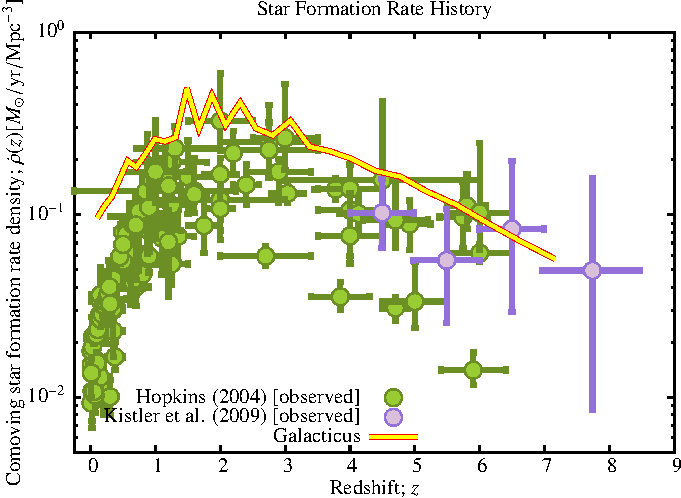
\includegraphics[scale=0.5]{r256/h100/NGenIC_10629/Plot_Star_Formation_History.pdf}\\
In Galacticus revision 821 the latest bug 'I think this was 
due to a missing limitation on the rate at which metals 
can be driven out of hot halos' is fixed and the 100h 
simulations runs again 


\item[11.05.2012]
Galacticus bug report 
\begin{verbatim}
Fatal error in ODEIV2_Solve():
ODE integration failed with status -1
...
\end{verbatim}
Link: \texttt{https://bugs.launchpad.net/galacticus/+bug/998007} \\ - 
occurs in \texttt{stages\_12\_h\_44} with h100. 

\item[10.05.2012]
Complete reinstallation of system since I had messed up my perl installation 
severely. Now the plotting scripts run again in revision 809. 

\item[08.05.2012]
Compiler flags for checking linking 
\begin{verbatim}
 -Wl,--verbose
\end{verbatim}
gives attempts/success/fail info about opening files. \\
New Galcticus revisions had problems compilingbut already 
fixed by Benson in rev 805. For consistency also update 
on pc122 so perl5 is still under construction \\

\item[02.05.2012]
Had to reinstall \texttt{perl5} (download + recompile) 
cause Galacticus plot routines did not work any more: 
Moreover I had to: 
\begin{verbatim}
$PERL5LIB=/usr/lib/perl5:/usr/local/lib/perl/5.12.4:
/usr/share/perl5:/usr/local/share/perl/5.12.4
$export PERL5LIB
\end{verbatim}
to get Galacticus itself compile again. \\

\item[25.04.2012]
Is low star formation rate in recent galacticus outputs 
related to missing IC redshift? (99 assumed) \\

\item[19.04.2012]
\texttt{stages\_52} simulation still shows extremely low 
star formation rate in history plot (Galacticus rev. 771) 
although also in Markus' converter-ed input file the box 
size of 44.8 Mpc is correct \\ 


\item[18.04.2012]
Comparison runs look principally nice but not equal - may be 
caused by different \texttt{linger.dat} \\
Comparison runs have to be redone since \texttt{grafic\_h70}
and \texttt{grafic\_h100} were 
not recompiled after changing \texttt{constr.f} and \texttt{grafic.inc} \\
2DO: check comparison runs, check new galacticus runs and 
restart rockstar job on MACH \\

\item[17.04.2012]
Started some comparison runs beweteen H=70.3 and H=100 with same 
\texttt{linger\_syn} parameters, same constraints and seeds \\
found nice program with GUI to look at hdf5 files and also to edit them, 
called \texttt{vitables} - big files take very long to load but 
once loaded it runs smoothly \\
not clear why the \texttt{stages\_52} simulation plots show 
such little star formation rate 
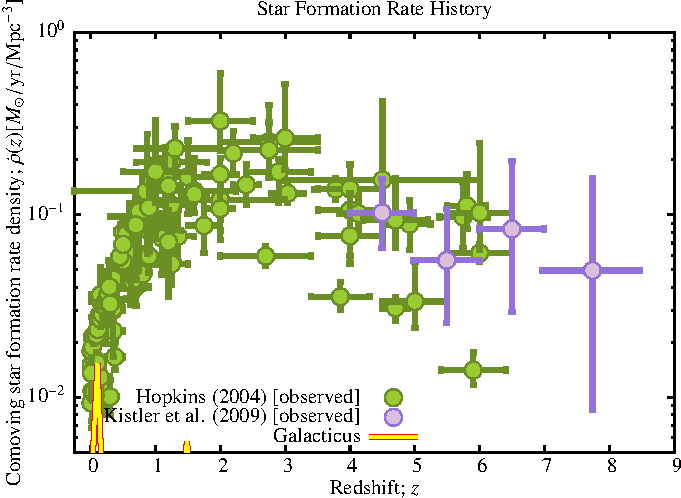
\includegraphics[scale=0.5]{r256/h100/stages_52/Plot_Star_Formation_History_small.pdf} \\

\item[16.04.2012]
re-doing the rockstar jobs that did not work on intel queue 
now on the AMD machines (\texttt{stages\_54dr5d5}) \\ 
512er run is being rockstarred on MACH (128 cores) faster than on 
our AMDs $\rightarrow$ quit job on astro-cluster \\

\item[12.04.2012]
Explicitly defining the ports when havin several server processes on
the frontend did not seem to work for the intel queue, all 
three rockstar jobs stopped working after some time \\

\item[04.04.2012]
E-Mail correspondence with Sabine Kreidl to Rockstar on MACH \\
Recompiled Gadget with \texttt{PLACEHIGHRESREGION=1} on and 
\texttt{PMGRID} resolution of 256 for 256er run \\

\item[03.04.2012]
Tried nonperiodic Gadget boundary conditions $\rightarrow$ leads 
to star-like patterns \\
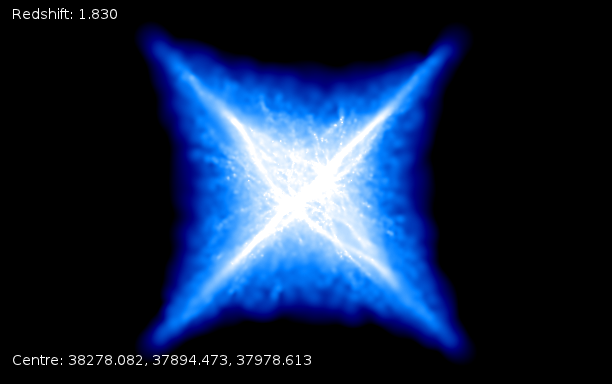
\includegraphics[scale=0.3]{r256/h100/nonperiodictest/drd5nonperiodic.png}
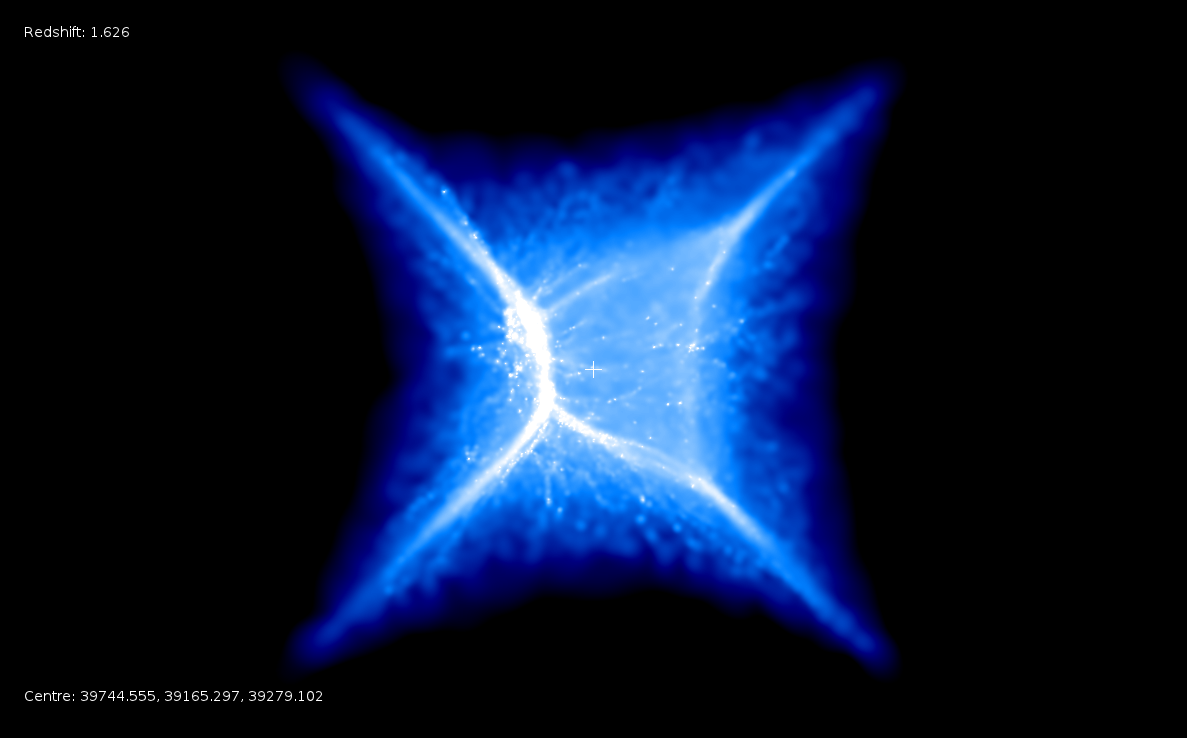
\includegraphics[scale=0.2]{r256/h100/nonperiodictest/stages20nonperiodic.png} \\


\item[02.04.2012]
Correspondence with Peter Behroozi concerning OpenMP parallelization
possibilities in Rockstar  $\rightarrow$ tried suggested loops 
and auto-parallelization. Jobs on intel machines freeze ... 

\item[27.03.2012] 
\texttt{512er\_major\_merger} Rockstar run is very slow even 
on 24 cores \\
\texttt{consistentree} has parameter \texttt{BOX\_DIVISIONS} which divides 
the box in this number cubed parts and makes \texttt{tree\_X\_Y\_Z.dat} 
output and is very very fast this way 
$\rightarrow$ have to rewrite reading routine in Markus' 
converter \\

\item[26.03.2012] 
Intel compiler auto-parallelization test runs on LEO3 
for converter v0.5 \\
$512^3$ runs produced Segfaults with Markus' converter 
v0.4 $\rightarrow$ fixed \\

\item[21.03.2012]
2DO: change virial radius reading in galaxcicusStart.xml 
to false and let intern value \\
powmes scripts, plotting scripts (spin, vrms) \\

\item[20.03.2012]
powemes installed 

\item[19.03.2012]
NGenIC starting redshift test, if corrected initial z leads to 
lower star formation rate did show, that suspicion was not 
proven. Other explanation has to be found. Vrms and Spin videos are 
in the works. 

\item[14.03.2012]
2DO: new stages simulations in Documentation 
(at least 46, 50, 51) \\
Script that makes *.pngs out of halo masses at all 
time steps is running over all simulations in r256  for 
comparison beweteen Bertschinger and NGenIC ICs \\
Rerun some Bertschinger ICs with updated linger.dat and 
spectral index $\neq$ 1 to see how this influences 
star formation rate (linger runs and runs) \\


\item[13.03.2012]
Unclear why all NGenIC simulations show much higher 
star formation and plot scripts yield different 
output files though the same .xml file as always 
is used 

\item[11.03.2012]
\texttt{NGenIC\_15039} produces "unreadable" output, 
is bein rerockstarred from scratch 
\begin{verbatim}
 +++ 
 Plot_Star_Formation_History.pl:
 +++ 
Useless use of private variable in void context at ../../perl//XMP/MetaData.pm line 16.
HDF5-DIAG: Error detected in HDF5 (1.8.4-patch1) thread 0:
  #000: ../../../src/H5D.c line 507 in H5Dget_type(): not a dataset
    major: Invalid arguments to routine
    minor: Inappropriate type
Error Calling PDL::IO::HDF5::Dataset::get: Can't get HDF5 Dataset type.
 at ../../perl//Galacticus/HDF5.pm line 88
HDF5-DIAG: Error detected in HDF5 (1.8.4-patch1) thread 0:
  #000: ../../../src/H5D.c line 507 in H5Dget_type(): not a dataset
    major: Invalid arguments to routine
    minor: Inappropriate type
Error Calling PDL::IO::HDF5::Dataset::get: Can't get HDF5 Dataset type.
 at ../../perl//Galacticus/HDF5.pm line 88
Illegal division by zero at Plot_Star_Formation_History.pl line 58.
\end{verbatim}

\item[09.03.2012]
strange error in 2 galacticus jobs \texttt{stages\_12} and 
\texttt{stages\_13}  $\rightarrow$ Markus' converter 
outdated with new consistenttrees? \\
\textbf{idea:} \texttt{drd5\_r256\_2} shows a major merger in progress 
$\rightarrow$ make a set of similar simulations with 
slightly different parameters \\
\textbf{idea:} make voids as constraints so that netto gravity is 
more centered towards overdensities \\

\item[08.03.2012]
add \texttt{nohup} to \texttt{./rockstar server\_ib.cfg} 
in \texttt{qsubrockstar.sh} and rename \texttt{rocky\_startscript}
to something recognizable 
\begin{verbatim}
83973 0.60500 wcon1Gy.st jan     r     11:01:23 astro14.astro-beowulf.      64        
83974 0.50500 rocky_star harre   r     13:14:22 astro-x4600-04.astro-beo     1        
83976 0.55421 stages_28_ harre   r     13:52:36 astro22.astro-beowulf.      32        
83977 0.55421 stages_29_ harre   r     13:56:35 astro25.astro-beowulf.      32        
83980 0.55421 stages_30_ harre   r     14:07:12 astro28.astro-beowulf.      32        
83984 0.55421 stages_31_ harre   r     14:14:23 astro31.astro-beowulf.      32        
83988 0.51611 rocky_star harre   r     14:49:20 astro-x4600-04.astro-beo     8        
83989 0.51611 rocky_star harre   r     14:50:54 astro-x4600-03.astro-beo     8        
83993 0.51611 rocky_star harre   r     15:12:52 astro-x4600-04.astro-beo     8        
83995 0.51611 rocky_star harre   r     15:16:43 astro-x4600-03.astro-beo     8        
83992 0.58278 c803_test_ markus  qw    14:54:54                             50        
83985 0.55421 stages_32_ harre   qw    14:14:31                             32        
83986 0.55421 stages_33_ harre   qw    14:14:41                             32     
\end{verbatim}
re-galacticussing \texttt{NgenIC\_15039} again since 
plotting scripts complain that there is no output for 
a=0 \\
2DO: test speedup of galacticus with 1,2,4,8 threads \\
\textbf{Rockstar} works if infiniband is forced with 
\texttt{PARALLEL\_IO\_SERVER\_INTERFACE = "ib0"}, 
the client IP address is indeed NOT necessary, 
client process is started with \texttt{auto-rockstar.cfg} \\
Gadget recompiled with newest openmpi version $\rightarrow$ 
should use infiniband now \\

\item[06.03.2012]
submitted 4 jobs with same seed but different constraints 
parameters \\
Memory agglomeration fix also on cluster + email to develooper \\
Wrote E-Mails to Rien de Weijgaert and Peter Behroozi \\
re-rockstarring \texttt{stages\_21} on my machine pc122  $\rightarrow$ 
dumped due to memory  \\

\item[02.03.2012]
re-galacticussing \texttt{NgenIC\_15039} cause 200 output redshifts 
lead to $>30$GB file + added luminosity output redshifts from 
Markus' .xml file \\
Peter answered and sent \texttt{consistent\_trees v0.99}, but problem 
persists - suspicion: Snapshotnames.dat must be changed (delete 
corresponding lines) for runs that have $<200$ outputs! \\
rockstar won't start any more ... network problem suspected \\


\item[01.03.2012]
wrote E-Mail to Peter concerning 
\texttt{find\_parents\_and\_cleanup: \\ find\_parents\_and\_cleanup.c:130}
problem \\
consistentree: \texttt{NgenIC\_15039}, galacticussing \\
restarted: \texttt{stages\_21} rockstarred auf AMD-04 \\
first $512^3$ simulation \texttt{NgenIC\_7755} finished successfully - lasted 
1 day on 64 cores \\
wrote E-mail to de Weijgaert concerning constrained ICs \\

\item[29.02.2012]
\texttt{stages\_12} re-rockstarred auf AMD-03 \\
\texttt{stages\_21} rockstarred auf AMD-04 - crashed \\
100Mpc $512^3$ jobs: 11410, 15725, 27036, 7755 \\
10 100Mpc ICs generated \\
\textbf{Note: try bigger volumes with NGen-IC} \\ 
added output redshifts derived from \texttt{gadget\_timer.txt} as 
parameter \texttt{outputRedshifts} in .xml file \\ 
Random seeds that do not create cluster like structures at 
32Mpc box: 589, 12170, 13610, 16604, 16749, 17362, 17433, 29666, 32223, 
17595, 22045, 3724, 3183, 4152, 7581, 8502, 10153, 10657, 22946, 14841, 
25060, 29468, 32634
\\
Random seeds that look a little interesting: 15039 $\rightarrow$ rockstarred 
on AMD-03 (finished), 26214 $\rightarrow$ rockstarred on AMD-04


\item[28.02.2012]
Successfully started some N-GenIC jobs for comparison of IC generation \\

\item[17.02.2012]
Discussion with Asmus about Stages Cluster $\rightarrow$ try more systematic 
approach to ICs 

\item[15.02.2012]
Galacticus revisision 708 - \texttt{drd5\_r256\_2} not fixed 
$\rightarrow$ E-Mail to Andrew \\
check tomorrow: Galacticus jobs \texttt{fuenfincr256\_1} and 
\texttt{drdx\_3\_r256} \\
\textbf{Note: think about / find a good method for common metadata} \\

\item[14.02.2012]
Wrote E-Mail to Bertschinger. \\

\item[13.02.2012]
Deleted some jobs I started yesterday because they had artificial crosses 
or were practically unconstrained \\
Third simulation \texttt{fuenfincr256\_1} ran through - Galacticus 
restart worked well! \\
\textbf{Note: IC with same seed but higher resolution do not yield the same 
simulation!} $\rightarrow$ started two more test runs from r128 sims to doublecheck \\
$\rightarrow$ Note from April 2012: different \texttt{linger.dat} 
suspected

\item[12.02.2012]
Updated Galacticus to revision 707 as suggested by Andrew and added parameter 
\texttt{hotHaloOutflowAngularMomentumAlwaysGrows} to xml file. \\
Two of four simulations ran through (copied hdf5 to transfer), 
two crashed $\rightarrow$ try to continue at saved states!

\item[10.02.2012]
wrote E-Mail to Andrew about performance problems and wavelenght computation error 
in \texttt{fuenfincr256\_1} \\
started some runs with higher central delta and broader smoothing lenghts, i.e. 
32/dx and 100/dx; all 128 resolution except second last one (same seed!): 
\begin{verbatim}
83492 0.60500 d31c_1_sta harre   r     02/10/2012 15:19:56 astro18  16        
83493 0.60500 d31c_2_sta harre   r     02/10/2012 15:20:37 astro29  16        
83494 0.60500 d31c_3_sta harre   r     02/10/2012 15:21:17 astro25  16        
83495 0.60500 d51c_sl100 harre   r     02/10/2012 15:23:21 astro31  16  
83496 0.54786 d3+3c_sl50 harre   r     02/10/2012 15:37:13 astro12  16        
83497 0.60500 d3+3c_sl50 harre   r     02/10/2012 15:39:16 astro30  32  
83498 0.60500 d15+3c_sl5 harre   r     02/10/2012 15:44:23 astro30  16        
\end{verbatim}

\item[09.02.2012]
\texttt{drd5\_r256} last written to hdf5 file feb 09, 05:07 \\
\texttt{fuenfincr256\_2} last written to hdf5 file feb 06, 03:28 \\
\texttt{drd5\_r256\_2} last written to hdf5 file feb 07, 00:50 \\

\item[02.02.2012]
\texttt{drdx\_h100\_128\_1} run has again severe consistency 
metric problem \\ $\rightarrow$ not clear why \\
upper python script does not work, was commented out again \\
plan: \textbf{move to python scripts in general in order to have
 easier arithmetic calculations} \\   
plan: create new folder structure and remove old simulations $\rightarrow$ done \\

\item[31.01.2012]
note: h=70.3 in galacticus xml input file is expected, consistent tree obviously implies it \\
$\rightarrow$ fixed: changed in markus parameter file for the converter and in xml file \\
$\rightarrow$ question: why not read out? \\
$\rightarrow$ python updateGalacticusStart.py from Markus 

\item[30.01.2012]
new consistenttree with vmax=20

\end{itemize}